\documentclass[aspectratio=169]{beamer}

% ---------- ENCODING & FONTS ----------
\usepackage[utf8]{inputenc}
\usepackage[T1]{fontenc}

% ---------- THEME & LOOK ----------
\usetheme{Madrid}
\usecolortheme{seahorse}
\usefonttheme{professionalfonts}
\setbeamertemplate{navigation symbols}{}
\setbeamercovered{transparent}
\setbeamertemplate{itemize items}[circle]
\setbeamertemplate{enumerate items}[default]
\setlength{\parskip}{0.25em}

% ---------- COLORS ----------
% Beamer already loads xcolor, so we just define our colors
\definecolor{accent}{RGB}{0,92,184}
\definecolor{soft}{RGB}{233,244,255}
\definecolor{lightred}{RGB}{245,210,210}
\setbeamercolor{structure}{fg=accent}
\setbeamercolor{title}{fg=white,bg=accent}
\setbeamercolor{frametitle}{fg=accent}
\setbeamercolor{block title}{bg=accent!12,fg=accent}
\setbeamercolor{block body}{bg=soft}

% ---------- PACKAGES ----------
\usepackage{booktabs}
\usepackage{amsmath, amssymb}
\usepackage{array}
\usepackage{multirow}
\usepackage{hyperref}
\hypersetup{colorlinks=true,linkcolor=accent,urlcolor=accent}

% ---------- SAFE TRANSITION FALLBACK ----------
\makeatletter
\@ifundefined{transfade}{\newcommand{\transfade}[1][]{}}{}
\makeatother

% ---------- PLACEHOLDER BOX FOR FIGURES ----------
\newcommand{\placeholderbox}[2][0.82\linewidth]{%
  \begin{center}
    \fbox{\begin{minipage}[c][0.46\textheight][c]{#1}
      \centering \vspace{0.3em}
      \textbf{#2}\\[0.6em]
      \emph{Insert figure/diagram here later.}
    \end{minipage}}
  \end{center}
}


% ---------- TITLE ----------
\title{\textbf{Monetary Policy \vspace{.5cm}\\  }}
\subtitle{ {\large ECON 101 - Macroeconomics}}
%\institute{UNBC}
\author{Muhebullah Karimzada}
\date{Winter 2026}


\begin{document}

% ============================================================
% TITLE
% ============================================================
\begin{frame}[plain]
  \titlepage
\end{frame}

% ============================================================
\begin{frame}{Chapter Outline}
\transfade
\begin{itemize}
  \item \textbf{11.1} What Is Monetary Policy?
  \item \textbf{11.2} The Money Market and the Bank of Canada’s Choice of Monetary Policy Targets
  \item \textbf{11.3} Monetary Policy and Economic Activity
  \item \textbf{11.5} A Closer Look at the Bank of Canada’s Setting of Monetary Policy Targets
\end{itemize}
\end{frame}

% ============================================================
\section{11.1 What Is Monetary Policy?}
% ============================================================

\begin{frame}{11.1 Learning Objective}
\transfade
\begin{block}{Goal}
Define monetary policy and describe the Bank of Canada’s monetary policy goals.
\end{block}
\begin{itemize}
  \item Build on the previous chapter on money and banking.
  \item Understand \textbf{what} the Bank of Canada (BoC) is trying to achieve.
  \item See \textbf{why} monetary policy matters for inflation, unemployment, and growth.
\end{itemize}
\end{frame}

\begin{frame}{What Is the Role of the Bank of Canada?}
\transfade
\begin{itemize}
  \item Created in \textbf{1934}.
  \item Main responsibility:
  \begin{itemize}
    \item conduct monetary policy “in the best interests of the economic life of the nation.”
  \end{itemize}
  \item Since World War II:
  \begin{itemize}
    \item the BoC has carried out an \textbf{active} monetary policy.
  \end{itemize}
  \item \textbf{Monetary policy}:
  \begin{itemize}
    \item actions the Bank of Canada takes to manage the \alert{money supply} and \alert{interest rates}
    \item in order to pursue \alert{macroeconomic policy goals}.
  \end{itemize}
\end{itemize}
\end{frame}

\begin{frame}{The Goals of Monetary Policy}
\transfade
\begin{itemize}
  \item The Bank of Canada pursues four main monetary policy goals:
\end{itemize}
\begin{table}[h]
\centering
\begin{tabular}{p{0.32\linewidth} p{0.6\linewidth}}
\toprule
\textbf{Goal} & \textbf{Meaning / Why it matters} \\
\midrule
Price stability & Keep inflation low and stable so money remains a reliable unit of account and store of value. \\
High employment & Keep the economy close to full employment, avoiding unnecessarily high unemployment. \\
Stability of financial markets and institutions & Ensure banks and financial markets function smoothly, avoiding crises that disrupt credit. \\
Economic growth & Support long-run growth in real GDP by providing a stable monetary environment. \\
\bottomrule
\end{tabular}
\end{table}
\end{frame}

\begin{frame}{Why These Goals Are Connected}
\transfade
\begin{itemize}
  \item In the long run:
  \begin{itemize}
    \item healthy growth requires price stability and a stable financial system.
  \end{itemize}
  \item In the short run:
  \begin{itemize}
    \item reducing inflation too aggressively can increase unemployment,
    \item easing too much to reduce unemployment can fuel inflation.
  \end{itemize}
  \item Monetary policy involves \alert{trade-offs}, especially in the short run.
\end{itemize}
\end{frame}

% ============================================================
\section{11.2 The Money Market and Policy Targets}
% ============================================================

\begin{frame}{11.2 Learning Objective}
\transfade
\begin{block}{Goal}
Describe the Bank of Canada’s monetary policy targets and explain how expansionary and contractionary policies affect the interest rate.
\end{block}
\begin{itemize}
  \item The BoC has \textbf{two main tools}:
  \begin{itemize}
    \item open market operations,
    \item lending to financial institutions.
  \end{itemize}
  \item These tools influence \textbf{monetary policy targets}:
  \begin{itemize}
    \item the money supply,
    \item the short-term interest rate (primary target).
  \end{itemize}
\end{itemize}
\end{frame}

\begin{frame}{Monetary Policy Tools and Targets}
\transfade
\begin{itemize}
  \item \textbf{Open market operations}:
  \begin{itemize}
    \item the BoC buys or sells government securities.
  \end{itemize}
  \item \textbf{Lending to financial institutions}:
  \begin{itemize}
    \item provides short-term funds to banks (standing liquidity facilities).
  \end{itemize}
  \item The BoC cannot directly control:
  \begin{itemize}
    \item the inflation rate,
    \item real GDP or unemployment.
  \end{itemize}
  \item Instead, it targets:
  \begin{itemize}
    \item the money supply, and especially
    \item a short-term nominal interest rate.
  \end{itemize}
\end{itemize}
\end{frame}

\begin{frame}{Figure 11.2 -- The Demand for Money }
\centering
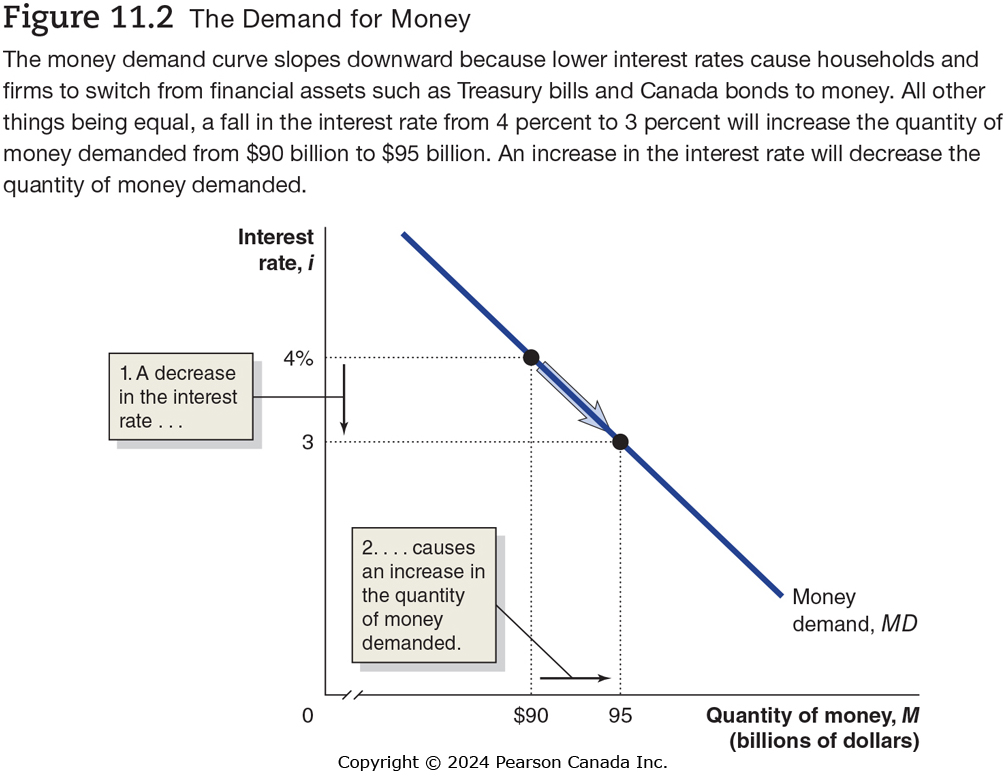
\includegraphics[width=0.6\linewidth]{Fig11-002}
\end{frame}

\begin{frame}{The Demand for Money}
\transfade
\begin{itemize}
  \item The BoC’s two monetary policy targets are \textbf{linked}:
  \begin{itemize}
    \item higher interest rates \(\Rightarrow\) lower quantity of money demanded.
  \end{itemize}
  \item Why?
  \begin{itemize}
    \item When interest rates are high, alternatives to holding money (e.g., bonds) look attractive.
    \item The \alert{opportunity cost} of holding money is higher.
  \end{itemize}
  \item Result:
  \begin{itemize}
    \item as the nominal interest rate rises, households and firms hold \textbf{less} money and more interest-bearing assets.
  \end{itemize}
\end{itemize}
\end{frame}

\begin{frame}{Figure 11.3 -- Shifts in the Money Demand Curve}
\centering
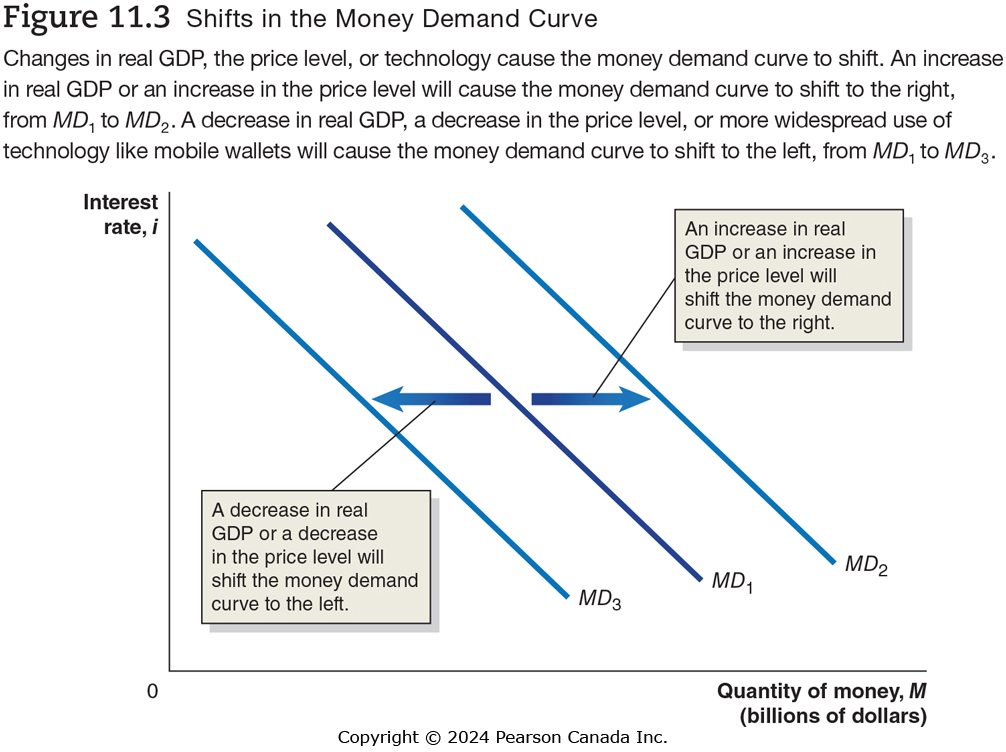
\includegraphics[width=0.6\linewidth]{Fig11-003}
\end{frame}

\begin{frame}{Shifts in Money Demand}
\transfade
\begin{itemize}
  \item Money demand depends on the \textbf{need to hold money} to pay for goods and services.
  \item If more transactions are taking place:
  \begin{itemize}
    \item higher real GDP,
    \item higher price level (more dollars needed per transaction),
  \end{itemize}
  \item then the demand for money is \textbf{higher}.
  \item Conversely:
  \begin{itemize}
    \item decreases in real GDP or the price level reduce money demand.
  \end{itemize}
\end{itemize}
\end{frame}

\begin{frame}{How the BoC Manages the Money Supply}
\transfade
\begin{itemize}
  \item To \textbf{increase} the money supply:
  \begin{itemize}
    \item the BoC \alert{buys} government securities,
    \item the sellers deposit the proceeds into bank accounts,
    \item banks make new loans, and the money supply \textbf{expands}.
  \end{itemize}
  \item To \textbf{decrease} the money supply:
  \begin{itemize}
    \item the BoC \alert{sells} government securities,
    \item buyers pay from their bank deposits,
    \item bank reserves fall, loans contract, and the money supply \textbf{shrinks}.
  \end{itemize}
\end{itemize}
\end{frame}

\begin{frame}{Figure 11.4 -- Increasing the Money Supply }
\centering
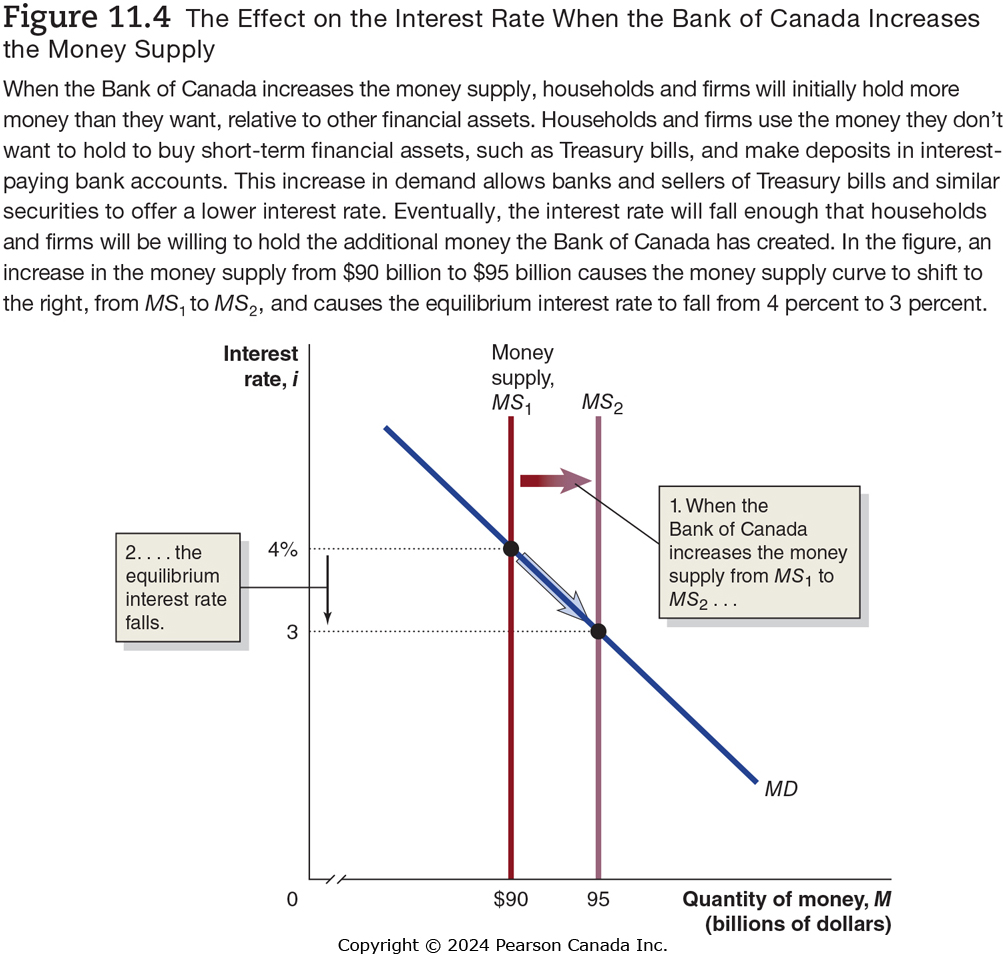
\includegraphics[width=0.5\linewidth]{Fig11-004}
\end{frame}

\begin{frame}{Effect of Increasing the Money Supply on Interest Rates}
\transfade
\begin{itemize}
  \item Assume, for simplicity, that the BoC can fully control the money supply:
  \begin{itemize}
    \item the money supply curve is a \textbf{vertical} line.
  \end{itemize}
  \item Equilibrium occurs where money demand intersects money supply.
  \item When the BoC increases the money supply:
  \begin{itemize}
    \item the vertical money supply curve shifts right,
    \item households and firms now hold more money than they want,
    \item they buy bonds and other assets,
    \item bond prices rise, and the short-term interest rate \textbf{falls}.
  \end{itemize}
\end{itemize}
\end{frame}

\begin{frame}{Figure 11.5 -- Decreasing the Money Supply}
\centering
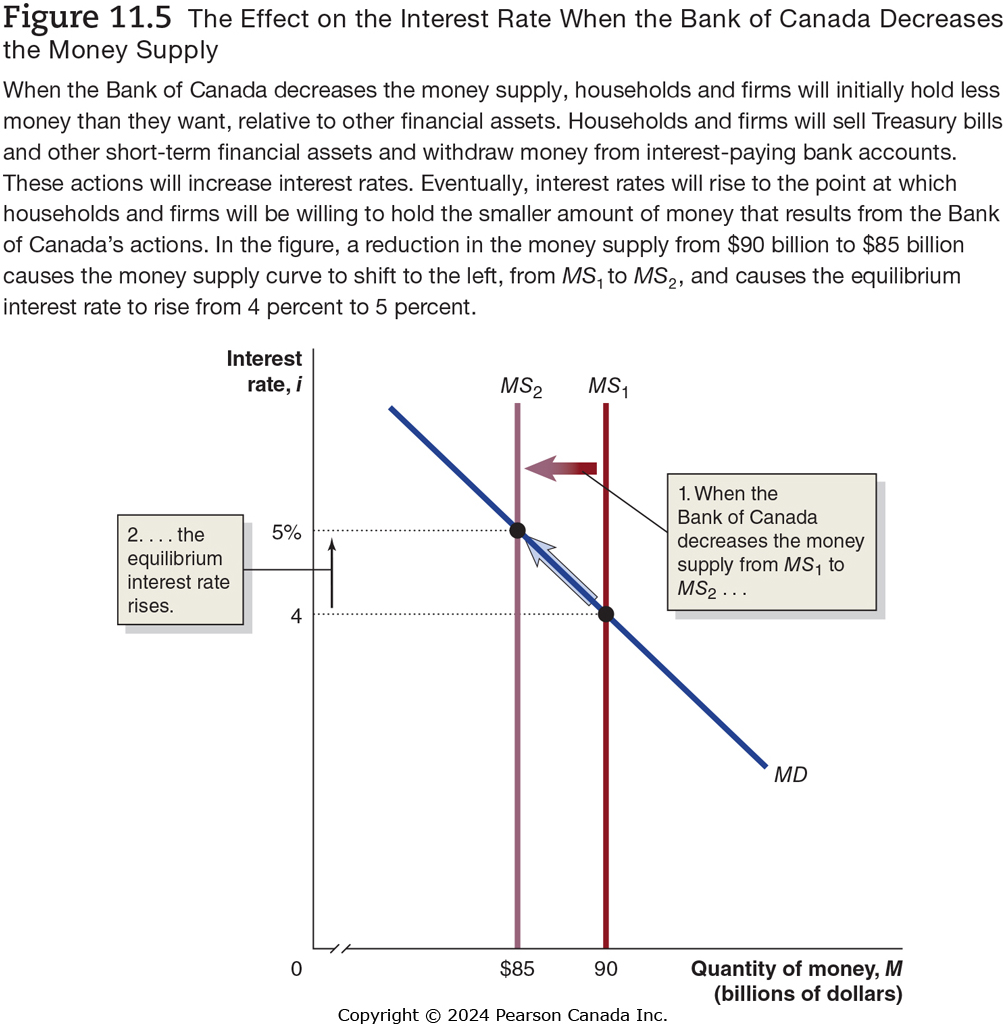
\includegraphics[width=0.48\linewidth]{Fig11-005}
\end{frame}

\begin{frame}{Effect of Decreasing the Money Supply on Interest Rates}
\transfade
\begin{itemize}
  \item When the BoC \textbf{lowers} the money supply (e.g., by selling Canada bonds):
  \begin{itemize}
    \item households and firms use money to buy the bonds,
    \item they are left with less money than they desire relative to other assets.
  \end{itemize}
  \item To attract and keep depositors, banks:
  \begin{itemize}
    \item offer higher interest rates on deposits.
  \end{itemize}
  \item Result:
  \begin{itemize}
    \item the short-term nominal interest rate \textbf{rises}.
  \end{itemize}
\end{itemize}
\end{frame}

\begin{frame}{A Tale of Two Interest Rates}
\transfade
\begin{itemize}
  \item We now have two models of interest rates:
  \begin{enumerate}
    \item \textbf{Loanable funds model} (Chapter 6)
      \begin{itemize}
        \item determines the \alert{long-term real} interest rate,
        \item relevant for firms’ capital investment and households building new homes.
      \end{itemize}
    \item \textbf{Money market model} (this chapter)
      \begin{itemize}
        \item determines the \alert{short-term nominal} interest rate,
        \item most relevant for the BoC, since changes in the money supply directly affect this rate.
      \end{itemize}
  \end{enumerate}
  \item Usually:
  \begin{itemize}
    \item long-term and short-term rates move together.
  \end{itemize}
\end{itemize}
\end{frame}

\begin{frame}{Choosing a Monetary Policy Target}
\transfade
\begin{itemize}
  \item The BoC can \textbf{target} either:
  \begin{itemize}
    \item a particular level of the money supply, or
    \item a particular short-term nominal interest rate.
  \end{itemize}
  \item In practice, it focuses on the \textbf{interest rate}.
  \item There are many interest rates; the key one is the:
  \begin{block}{Overnight interest rate}
    The interest rate banks charge each other for overnight loans.
  \end{block}
  \item The BoC announces its \textbf{target overnight rate} on eight fixed dates each year and uses open market operations to keep the actual overnight rate close to target.
\end{itemize}
\end{frame}

\begin{frame}{Figure 11.6 -- Overnight Rate Targeting, 1960–2022}
\centering
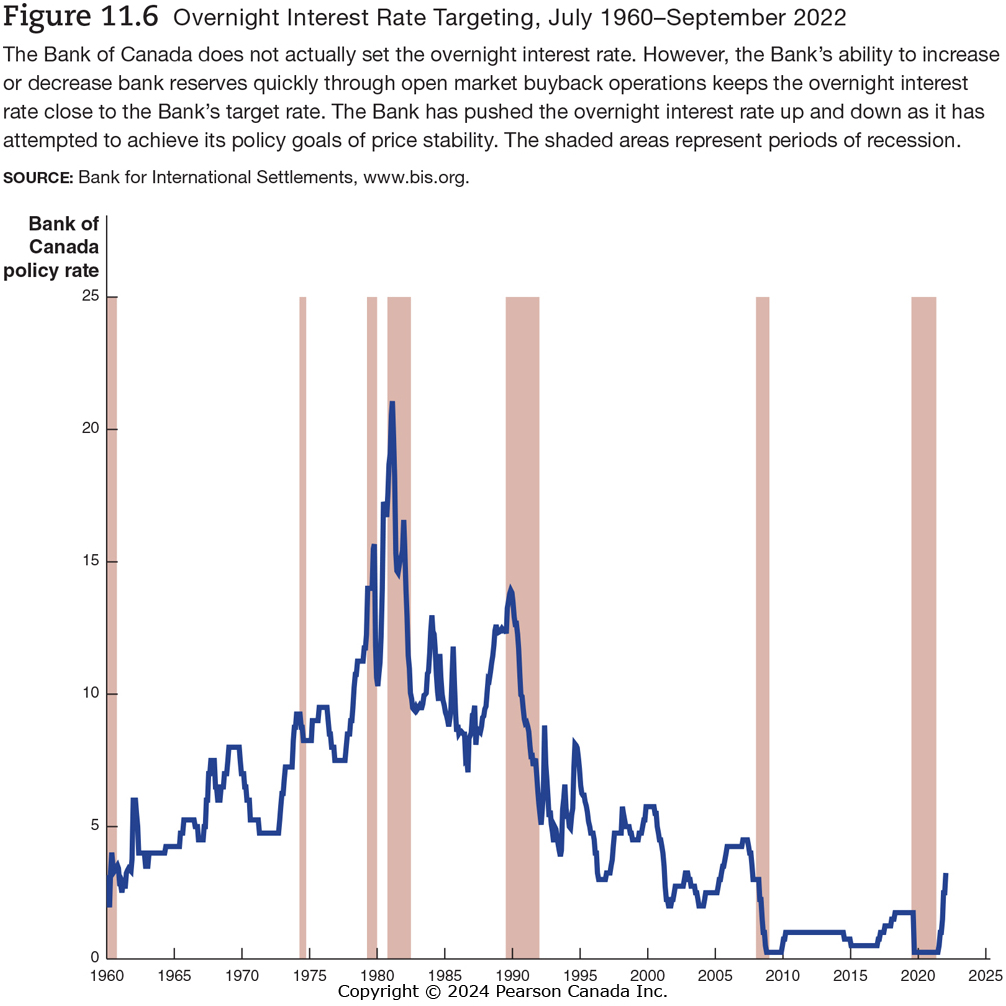
\includegraphics[width=0.48\linewidth]{Fig11-006}
\end{frame}

\begin{frame}{Overnight Rate and the Business Cycle}
\transfade
\begin{itemize}
  \item Over the years, the BoC has \textbf{raised and lowered} the overnight rate to achieve its goals.
  \item During:
  \begin{itemize}
    \item the 2007–2009 financial crisis,
    \item and the COVID-19 recession in 2020,
  \end{itemize}
  \item the BoC \textbf{cut} the target overnight rate several times.
  \item A change in the overnight rate has:
  \begin{itemize}
    \item a larger effect on short-term interest rates,
    \item but still influences longer-term rates and broader financial conditions.
  \end{itemize}
\end{itemize}
\end{frame}

% ============================================================
\section{11.3 Monetary Policy and Economic Activity}
% ============================================================

\begin{frame}{11.3 Learning Objective}
\transfade
\begin{block}{Goal}
Use aggregate demand and aggregate supply graphs to show the effects of monetary policy on real GDP and the price level.
\end{block}
\begin{itemize}
  \item The BoC’s ability to affect real GDP depends on its ability to influence \textbf{long-term real interest rates}.
  \item It uses the \textbf{overnight rate} (a short-term nominal rate) as a tool.
  \item We \alert{assume} here that changes in the overnight rate can affect long-term real interest rates.
\end{itemize}
\end{frame}

\begin{frame}{How Interest Rates Affect Aggregate Demand}
\transfade
\begin{itemize}
  \item Interest rates affect:
  \begin{enumerate}
    \item \textbf{Consumption}
      \begin{itemize}
        \item Lower rates encourage buying on credit, especially durables (cars, appliances).
        \item Lower rates reduce the reward to saving.
      \end{itemize}
    \item \textbf{Investment}
      \begin{itemize}
        \item Lower rates make it cheaper for firms to finance new capital (machines, factories).
        \item Lower rates make stocks more attractive, easing firms’ equity financing.
        \item Lower rates encourage residential construction.
      \end{itemize}
    \item \textbf{Net exports}
      \begin{itemize}
        \item Higher Canadian interest rates attract foreign funds.
        \item The Canadian dollar appreciates, making exports more expensive and imports cheaper.
        \item Net exports fall when domestic interest rates rise, and increase when they fall.
      \end{itemize}
  \end{enumerate}
\end{itemize}
\end{frame}

\begin{frame}{Figure 11.7 -- Expansionary Monetary Policy (1 of 2) }
\centering
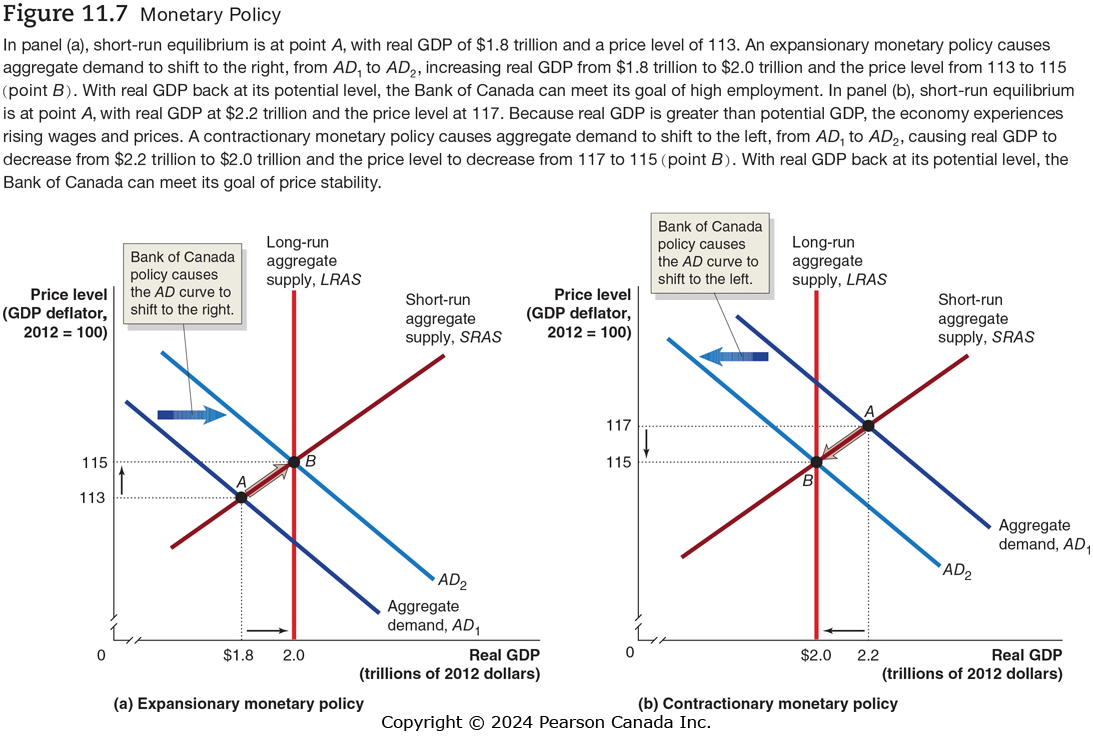
\includegraphics[width=0.65\linewidth]{Fig11-007}
\end{frame}

\begin{frame}{Expansionary Monetary Policy}
\transfade
\begin{itemize}
  \item \textbf{Expansionary monetary policy}:
  \begin{itemize}
    \item BoC actions that \alert{decrease} interest rates to \alert{increase} real GDP.
  \end{itemize}
  \item This is appropriate when:
  \begin{itemize}
    \item short-run equilibrium real GDP is \textbf{below} potential GDP (recession).
  \end{itemize}
  \item Mechanism:
  \begin{itemize}
    \item lower interest rates \(\Rightarrow\) higher consumption, investment, and net exports,
    \item \(\Rightarrow\) aggregate demand (AD) shifts to the \textbf{right},
    \item \(\Rightarrow\) real GDP and employment increase.
  \end{itemize}
\end{itemize}
\end{frame}



\begin{frame}{Contractionary Monetary Policy}
\transfade
\begin{itemize}
  \item Sometimes the economy produces \textbf{above} potential GDP:
  \begin{itemize}
    \item unemployment is very low,
    \item inflationary pressures are building.
  \end{itemize}
  \item \textbf{Contractionary monetary policy}:
  \begin{itemize}
    \item BoC actions that \alert{increase} interest rates to \alert{reduce} inflation.
  \end{itemize}
  \item Why intentionally reduce real GDP?
  \begin{itemize}
    \item The BoC is focused on \textbf{long-run growth}.
    \item If inflation becomes a problem, tightening policy helps maintain \alert{price stability}.
  \end{itemize}
\end{itemize}
\end{frame}

\begin{frame}{Can the BoC Eliminate Recessions?}
\transfade
\begin{itemize}
  \item In textbook diagrams, the BoC:
  \begin{itemize}
    \item knows exactly how far to shift AD,
    \item and manages to shift AD by precisely that amount.
  \end{itemize}
  \item In reality, monetary policy is much harder:
  \begin{itemize}
    \item the BoC does \textbf{not} know the exact size of shocks,
    \item the economy is always hit by new shocks,
    \item the effects of policy occur with \textbf{lags}.
  \end{itemize}
  \item Completely eliminating recessions is unrealistic.
  \item The best the BoC can do is to make recessions \textbf{milder} and \textbf{shorter}.
\end{itemize}
\end{frame}

\begin{frame}{Data Lags and Policy Lags}
\transfade
\begin{itemize}
  \item \textbf{Data lag}:
  \begin{itemize}
    \item key statistics (GDP, unemployment, inflation) are available only with a delay.
    \item Example: GDP for the 4th quarter of 2021 (Oct–Dec) is only published in March 2022.
  \end{itemize}
  \item \textbf{Policy lag}:
  \begin{itemize}
    \item it takes time for the BoC to recognize problems and implement policy changes.
  \end{itemize}
  \item \textbf{Effect lag}:
  \begin{itemize}
    \item it takes time for interest rate changes to affect spending, AD, and GDP.
  \end{itemize}
\end{itemize}
\end{frame}

\begin{frame}{Figure 11.8 -- Poorly Timed Monetary Policy}
\centering
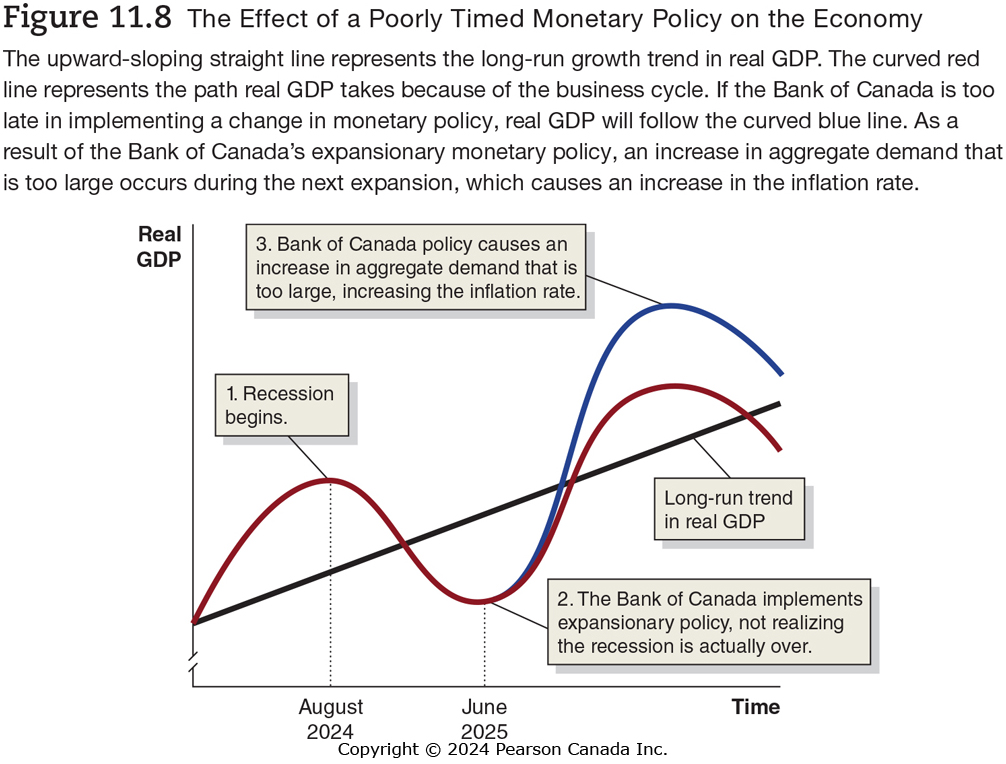
\includegraphics[width=0.6\linewidth]{Fig11-008}
\end{frame}

\begin{frame}{What If Policy Is Poorly Timed?}
\transfade
\begin{itemize}
  \item Suppose a recession begins in August 2020.
  \item Because of data and decision lags:
  \begin{itemize}
    \item the BoC only recognizes it later.
  \end{itemize}
  \item Assume the BoC starts expansionary policy in June 2021, when:
  \begin{itemize}
    \item the recession has already ended and recovery is underway.
  \end{itemize}
  \item Keeping interest rates low for too long:
  \begin{itemize}
    \item pushes real GDP \textbf{far above} potential,
    \item creates \textbf{high inflation},
    \item and makes the next recession more severe when policy eventually tightens.
  \end{itemize}
\end{itemize}
\end{frame}

\begin{frame}{Figure 11.9 -- Expansionary and Contractionary Policies }
\centering
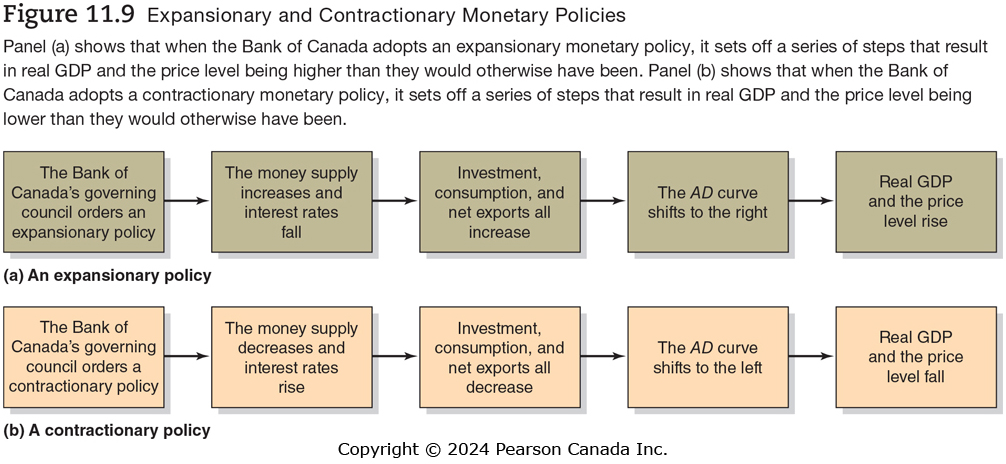
\includegraphics[width=0.9\linewidth]{Fig11-009}
\end{frame}

\begin{frame}{Summary: Expansionary vs. Contractionary Policy}
\transfade
\begin{itemize}
  \item \textbf{Expansionary policy:}
  \begin{itemize}
    \item lowers interest rates,
    \item increases C, I, and NX,
    \item shifts AD right,
    \item raises real GDP and employment,
    \item may increase inflation.
  \end{itemize}
  \item \textbf{Contractionary policy:}
  \begin{itemize}
    \item raises interest rates,
    \item reduces C, I, and NX,
    \item shifts AD left,
    \item reduces inflationary pressures,
    \item may temporarily reduce real GDP and increase unemployment.
  \end{itemize}
\end{itemize}
\end{frame}

% ============================================================
\section{11.5 Setting Monetary Policy Targets}
% ============================================================

\begin{frame}{11.5 Learning Objective}
\transfade
\begin{block}{Goal}
Discuss the Bank of Canada’s setting of monetary policy targets.
\end{block}
\begin{itemize}
  \item Should the BoC target the money supply or the interest rate?
  \item What simple rules have economists proposed?
  \item How does \textbf{inflation targeting} fit into modern practice?
\end{itemize}
\end{frame}

\begin{frame}{Should the BoC Target the Money Supply?}
\transfade
\begin{itemize}
  \item In normal times, the BoC targets the \textbf{overnight rate}.
  \item Some economists asked: should it target the \textbf{money supply} instead?
  \item \textbf{Monetarists}, led by Milton Friedman, argued “yes”:
  \begin{itemize}
    \item advocate a \alert{monetary growth rule}:
    \item increase the money supply at about the long-run rate of real GDP growth.
  \end{itemize}
  \item They argued:
  \begin{itemize}
    \item active countercyclical policy might destabilize the economy,
    \item a simple rule would provide more stability.
  \end{itemize}
\end{itemize}
\end{frame}

\begin{frame}{Why Monetarism Lost Influence}
\transfade
\begin{itemize}
  \item Monetarism was popular in the 1970s.
  \item Since the 1980s, the link between:
  \begin{itemize}
    \item the money supply and real GDP,
    \item the money supply and inflation,
  \end{itemize}
  \item has weakened.
  \item For example, M1+ often changes “wildly,” but:
  \begin{itemize}
    \item real GDP and inflation do not move in the same way.
  \end{itemize}
  \item As a result, support for following a strict monetary growth rule has declined.
\end{itemize}
\end{frame}

\begin{frame}{Figure 11.12 -- Can the BoC Target Both Money and Interest?}
\centering
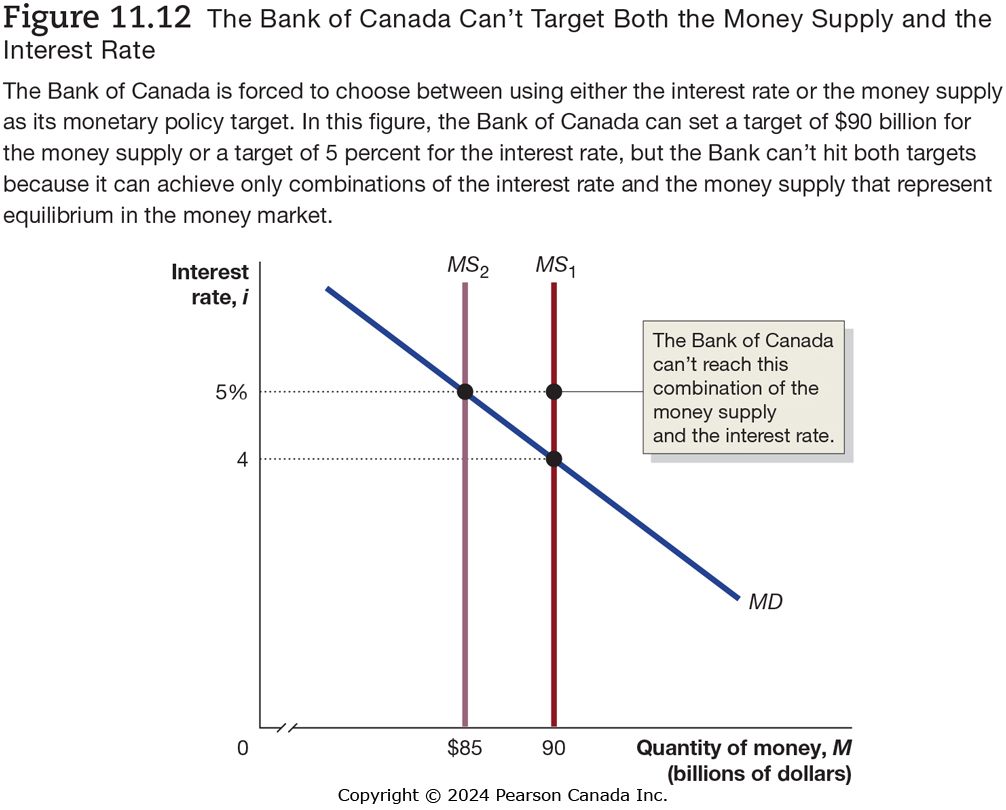
\includegraphics[width=0.6\linewidth]{Fig11-012}
\end{frame}

\begin{frame}{Why the BoC Can’t Target Both M and i}
\transfade
\begin{itemize}
  \item It might seem attractive to:
  \begin{itemize}
    \item target both the money supply and the interest rate.
  \end{itemize}
  \item But they are linked through the money demand curve:
  \begin{itemize}
    \item decreasing the money supply raises the equilibrium interest rate,
    \item increasing the money supply lowers the equilibrium interest rate.
  \end{itemize}
  \item Therefore:
  \begin{itemize}
    \item the BoC cannot independently fix both the money supply and the interest rate.
    \item It must choose one as its primary target.
  \end{itemize}
\end{itemize}
\end{frame}

\begin{frame}{The Taylor Rule (1 of 2)}
\transfade
\begin{itemize}
  \item The \textbf{Taylor rule} (John Taylor, Stanford) links the central bank’s target overnight rate to macroeconomic conditions.
  \item A generic version:
  \[
    i_{t} = r^{*} + \pi_{t}
      + \frac{1}{2}(\pi_{t} - \pi^{*})
      + \frac{1}{2} \left( \frac{Y_{t} - Y^{*}_{t}}{Y^{*}_{t}} \right),
  \]
  where:
  \begin{itemize}
    \item \(i_{t}\): target nominal overnight rate,
    \item \(r^{*}\): long-run real interest rate,
    \item \(\pi_{t}\): current inflation rate,
    \item \(\pi^{*}\): target inflation rate,
    \item \(Y_{t}\): real GDP,
    \item \(Y^{*}_{t}\): potential GDP.
  \end{itemize}
\end{itemize}
\end{frame}

\begin{frame}{The Taylor Rule (2 of 2)}
\transfade
\begin{itemize}
  \item The weights of \(1/2\) on:
  \begin{itemize}
    \item the \textbf{inflation gap} \((\pi_{t} - \pi^{*})\),
    \item and the \textbf{output gap} \(\left( \frac{Y_{t} - Y^{*}_{t}}{Y^{*}_{t}} \right)\),
  \end{itemize}
  \item would differ if the BoC were more or less concerned about inflation or output.
  \item In the Taylor rule:
  \begin{itemize}
    \item the coefficient on the inflation gap is greater than zero,
    \item so if inflation rises by 1 percentage point, the overnight rate rises by \textbf{more than} 1 percentage point.
  \end{itemize}
  \item This is the \textbf{Taylor principle}:
  \begin{itemize}
    \item to stabilize the economy, monetary policy must raise the real interest rate when inflation rises.
  \end{itemize}
  \item Many economists see the Taylor rule as a useful \alert{benchmark} for analyzing overnight rate decisions.
\end{itemize}
\end{frame}

\begin{frame}{Inflation Targeting}
\transfade
\begin{itemize}
  \item \textbf{Inflation targeting}:
  \begin{itemize}
    \item a framework in which the central bank announces an explicit target for the inflation rate.
  \end{itemize}
  \item By the 1980s, many central banks had adopted inflation targets.
  \item For example:
  \begin{itemize}
    \item the BoC announces a target range for inflation,
    \item the U.S. Federal Reserve publicly announced a 2\% inflation target.
  \end{itemize}
\end{itemize}
\end{frame}

\begin{frame}{Why Use Inflation Targeting?}
\transfade
\begin{itemize}
  \item Inflation targeting:
  \begin{itemize}
    \item informs the public about the BoC’s objectives,
    \item provides an \alert{anchor} for inflation expectations,
    \item increases accountability for the central bank.
  \end{itemize}
  \item Economists and policymakers debate whether inflation targets improve policy, but:
  \begin{itemize}
    \item by 2021, many central banks had adopted inflation targeting,
    \item but no major central bank had adopted \textbf{nominal GDP targeting}.
  \end{itemize}
\end{itemize}
\end{frame}

% ============================================================
\section*{Chapter Summary}
% ============================================================

\begin{frame}{Summary}
\transfade
\begin{itemize}
  \item Monetary policy: actions by the Bank of Canada to manage the money supply and interest rates in pursuit of:
  \begin{itemize}
    \item price stability, high employment, financial stability, and economic growth.
  \end{itemize}
  \item The BoC uses open market operations and lending to financial institutions to influence:
  \begin{itemize}
    \item the money supply and,
    \item primarily, the overnight interest rate.
  \end{itemize}
  \item Changes in interest rates affect aggregate demand through consumption, investment, and net exports.
  \item Expansionary policy lowers interest rates to raise real GDP toward potential; contractionary policy raises rates to curb inflation.
  \item The BoC cannot target both the money supply and the interest rate simultaneously.
  \item Rules such as the Taylor rule and frameworks like inflation targeting help guide and communicate monetary policy decisions.
\end{itemize}
\end{frame}

\begin{frame}
\centering
\Huge \textbf{Thank you!}
\end{frame}

\end{document}
